\documentclass[12pt]{article}
\usepackage{geometry}
\usepackage{graphicx} % 插图
\usepackage{float} % 插图位置固定
\usepackage{amsmath} % 文字加粗
\usepackage[UTF8]{ctex} %中文宏包
\setCJKmainfont{SimSun}
\usepackage{fontspec} %引入字体设置宏包
\setmainfont{Times New Roman}
\usepackage{indentfirst} %首行缩进
\usepackage{listings} %代码
\usepackage{color} %字体颜色
\usepackage{subfigure}  %插入多图时用子图显示的宏包

\usepackage{minted} %代码
\usemintedstyle{vs}


%\usepackage{fancyhdr} %页眉页脚
%\pagestyle{fancy} 
%\fancyhf{}
%\lhead{数字图像处理}
%\chead{Noise Reduction Using a Median Filter}
%\rhead{张青铭 \quad 3200105426}
%\renewcommand{\headrulewidth}{0pt}
%图片路径
\graphicspath{ {figures/} }

%页面格式
\geometry{a4paper,
left=20mm,
right=20mm,
top=20mm,
bottom=20mm }

\title{{\Huge{\textbf{数字图像处理}}}\\基于昇腾CANN的推理应用开发——黑白图像上色}
\author{信息与电子工程学院\quad 信息工程 \quad 3200105426\\张青铭}
\date{\today}

\begin{document}
\maketitle
\section{实验内容及目标}
\subsection{实验内容}
本实验主要介绍了基于昇腾CANN平台的黑白图像上色应用的开发方法。该应用选用的是colorization模型,以黑白图片作为输入,对黑白图像上色,并把预测的结果保存为彩色图片。通过本实验,您可以了解如何在昇腾平台上实现一个基于colorization模型的推理应用。

\subsection{实验目标}
1.掌握一个基于昇腾CANN平台的推理应用的基本结构。

2.理解colorization模型的网络结构及其数据预处理/后处理方式。
\section{网络结构}
黑白图像上色模型原理如下图所示,对物件(包括背景色)(L通道代表的灰度图)使用卷积运算提取特征,然后同样用卷积进行分类,从而尝试给出对灰度图片每个像素点的色彩预期(ab通道)。将ab通道的值resize到原始图片宽高并与L通道叠加后,转为RGB图片即可得到彩色图像。

其中模型的输入为Lab图像色域中分离出的L通道的数据,数据shape为(224,224,1),模型的输出为ab通道的数据,数据shape为(56,56,2)。
\begin{figure}[H]
	\centering
	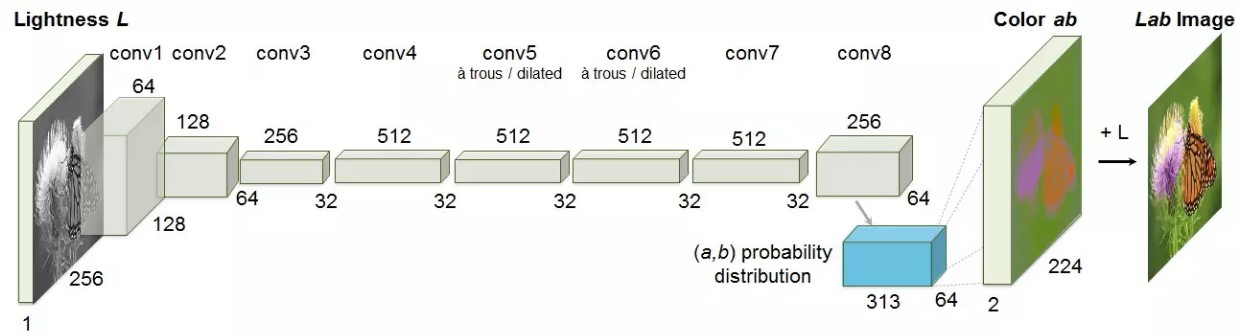
\includegraphics[width=0.8\linewidth]{figures/net}
	\caption{网络结构}
\end{figure}

\section{代码实现}
\begin{minted}[frame=lines,tabsize=4,python3,baselinestretch=0.85]{python}
import sys
import os
from IPython.core.interactiveshell import InteractiveShell
InteractiveShell.ast_node_interactivity = "all" 

home_path = !echo ${HOME}
sys.path.append(os.path.join(home_path[0] , "jupyter-notebook/"))
print('System init success.')

# atlas_utils是本团队基于pyACL封装好的一套工具库,如果您也想引用的话,请首先将
# https://gitee.com/ascend/samples/tree/master/python/common/atlas_utils
# 这个路径下的代码引入您的工程中
from atlas_utils.acl_resource import AclResource
from constants import *
from acl_model import Model

#创建一个AclResource类的实例
acl_resource = AclResource()
#AscendCL资源初始化(封装版本)
acl_resource.init()

# 上方“init”方法具体实现(仅供参考),请阅读“init()”方法,观察初始化和运行时资源申请的详细操作步骤
def init(self):
    """
    Init resource
    """
    print("init resource stage:")
    ret = acl.init()
    utils.check_ret("acl.init", ret)
    #指定用于运算的Device
    ret = acl.rt.set_device(self.device_id)
    utils.check_ret("acl.rt.set_device", ret)
    print("Set device n success.")

    #显式创建一个Context
    self.context, ret = acl.rt.create_context(self.device_id)
    utils.check_ret("acl.rt.create_context", ret)

    #创建一个Stream
    self.stream, ret = acl.rt.create_stream()
    utils.check_ret("acl.rt.create_stream", ret)

    #获取当前昇腾AI软件栈的运行模式
    #0:ACL_DEVICE,表示运行在Device的Control CPU上或开发者版上
    #1:ACL_HOST,表示运行在Host CPU上
    self.run_mode, ret = acl.rt.get_run_mode()
    utils.check_ret("acl.rt.get_run_mode", ret)

    print("Init resource success")

#请阅读下方代码,观察释放运行时资源的详细操作步骤
def __del__(self):
    print("acl resource release all resource")
    resource_list.destroy()
    
    #调用acl.rt.destroy_stream接口释放Stream
    if self.stream:
        acl.rt.destroy_stream(self.stream)
        print("acl resource release stream")
        
    #调用acl.rt.destroy_context接口释放Context
    if self.context:
        acl.rt.destroy_context(self.context)
        print("acl resource release context")
    
    #调用acl.rt.destroy_context接口释放Context
    acl.rt.reset_device(self.device_id)
    acl.finalize()
    print("Release acl resource success")
\end{minted}

\section{实验结果}
黑白图像上色结果如下:
\begin{figure}[H]
	\centering
	\subfigure[黑白图像]{
		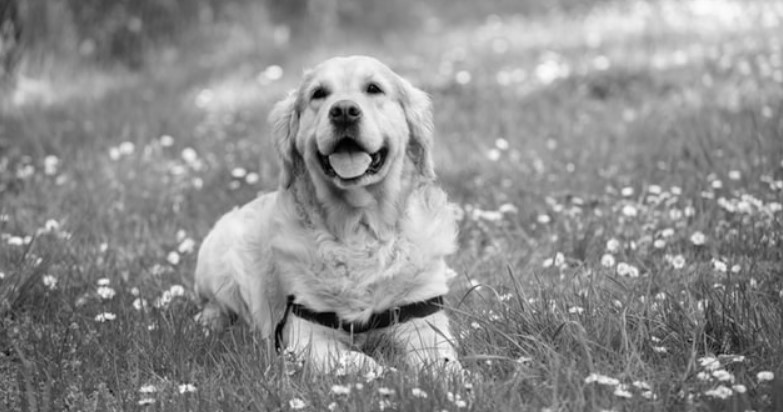
\includegraphics[width=0.4\linewidth]{figures/dog1}
	}
	\subfigure[上色图像]{
		
\includegraphics[width=0.4\linewidth]{figures/dig2}
	}
	\caption{黑白图像上色}
\end{figure}

\end{document}
